\chapter{MR-Cube 实现分析}

本章节中将对 \cite{nandi2011distributed} 中提出的 MR-Cube 进行分析,包括它的主要贡献和存在的不足。

\section{数据集}

在接下来的章节中需要数据集作为例子,因此这里先说明作为例子的数据集。数据集的表结构如图 \ref{dataset_table} 所示。表中共有 6 个维属性,分别是 country,state,city,topic,category,subcategory。其中\textless country, state, city\textgreater 是具有层次型的,同理\textless topic, category, subcategory\textgreater 也是具有层次性的。因此在 GroupBy 时,GroupBy(country, state, topic) 和 GroupBy(state, topic)是等价的。并且不会出现 GroupBy(country, city, topic) 这样的跨越层次的操作。

该数据集对应的 lattice 如图 \ref{dataset_lattice} 所示。图中的 ``*" 表示不需要聚合的属性。因为数据集具有层次型,因此lattice与上一章中看到的有所不同。上一章中提到,若有 D 个维属性,则 lattice 中有${2}^{D}$ 个节点,但由于这个数据集具有层次性,因此节点数有所减少。例如对于 (country, state, city) 这3个属性的 GroupBy,仅有 3 种结果,即 GroupBy(country),GroupBy(country, state)或 GroupBy(state) 以及 GroupBy(country, state, city)或 GroupBy(city)。


\begin{figure}[!htb]
\centering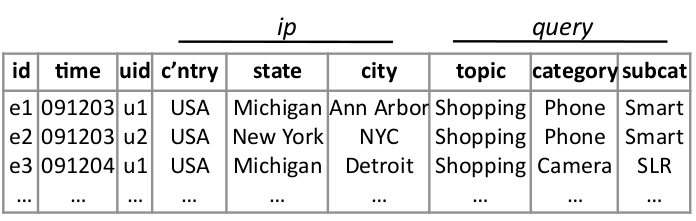
\includegraphics[width=3.5in]{picture/ch_datacube_mr/dataset_table} 
\caption{数据集的表结构}\label{dataset_table} 
\end{figure} 

\begin{figure}[!htb]
\centering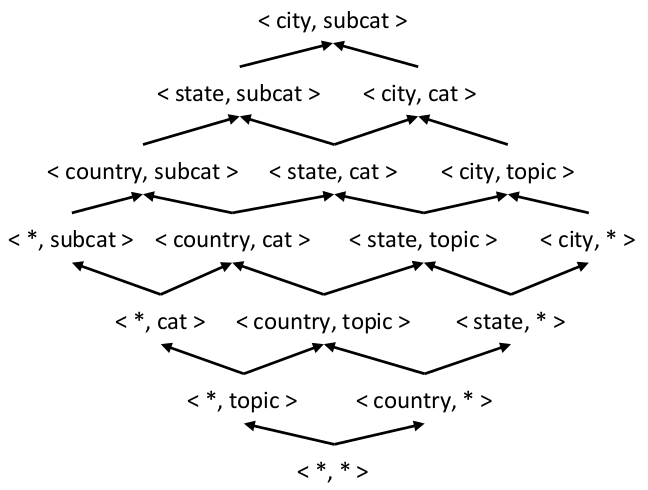
\includegraphics[width=3in]{picture/ch_datacube_mr/dataset_lattice} 
\caption{数据集的lattice}\label{dataset_lattice} 
\end{figure} 

在之后的章节中,将使用 \cite{nandi2011distributed} 中 region 与 group 的概念。region 指 lattice 中的每个节点,也即一种 GroupBy 的类型。group 指 region 中有具体值的 GroupBy。如 e1 和 e2 这两条记录,就可能属于 group(*,*,*,Shopping,Phone,*),而这个 group 则属于 (*,*,*,topic,category,*) 这个region。

\section{Naive 算法}

使用 MapReduce 计算 Data Cube,可以使用多次 MapReduce 计算各个 GroupBy,然后再将结果合并。但若计算资源较为充足的情况下,可使用一次 MapReduce 计算所有的 GroupBy,令计算资源被充分地使用。

图 \ref{naive_cube} 为 Naive 算法的实现。例如上述的数据集共有16个 region,那么对于输入的每一条记录,将其映射成对应的所有 group,并且与度量属性的值组成 key-value 作为 map 的输出。相同 key 值的数据将分派到同一个 reduce 上,也即相同 group 值的数据被分派到同一个 reduce 上,再进行聚合计算。例如输入的一条记录为 (e1, 091203, u1, USA, New Youk, NYC, Shopping, Phone, Smart),度量函数为 COUNT(DISTINCT(uid))。那么对于每一条记录,map 都输出 16 个 ([group value], [uid]) 的key-value,分别为([*,*], [u1]), ([*,Smart],[u1]), ([USA, *], [u1])等等。

\begin{figure}[!htb]
\centering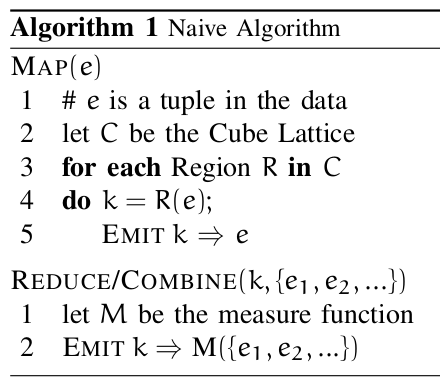
\includegraphics[width=3in]{picture/ch_datacube_mr/naive_cube} 
\caption{Naive 算法计算 Data Cube}\label{naive_cube} 
\end{figure} 

Naive的方法实现起来非常简单,对于较小的数据集也有很好的效果,但是随着数据集规模的增大,Naive的方法也存在不足,主要包括以下两个方面。

\begin{itemize}

\item \textbf{中间数据过多}

若 lattice 中的 region 数量为 $|C|$,数据集的大小为 $|D|$,则中间数据的数据量为 $|C|\times |D|$。随着维属性的增加,与层次的加深,中间数据的数据量则会巨增,必然导致 map 阶段有大量的磁盘 I/O,以及 shuffle(sort) 阶段有大量的数据需要排序,对整体的效率有非常大的影响。

\item \textbf{超大group}

在 mapreduce 计算中,总体的计算时间是由计算时间最长的 reduce 决定。因此若各个 reduce 分配到的要计算的数据量差异较大时,会导致某些 reduce 运行时间远大于其他 reduce。 在 Naive 的计算方法中,相同 group 值的数据会在一个 reduce 中计算,当这个 group 很大时,例如 lattice 中处于底层的 region 中的 group 相对就会较大,那么其他处理小 group 的 reduce 因为较早处理完数据,可能会空闲等待,甚至重新启动大 group 的计算,但重启计算效果往往并不佳,最终导致整个 mapreduce 的计算时间过长。

\end{itemize}

针对以上两个问题,MR-Cube提出了相应的解决方案。

\section{MR-Cube}

\subsection{整体性度量的划分}

对于大 group 的问题,我们可以将一个大 group 划分成多个子 group,这些子 group 分发到各个 reduce 上计算,即可解决 reduce 计算数据量不均匀的问题。但是并不是所有数据都可以随意划分,这个会受到度量函数的影响。

在第二章的准备知识中有提到,度量函数分为分布式度量函数、线性度量函数和整体性度量函数。对于前两种度量而言,数据确实可以划分,并且可以随意划分,因为无论数据怎么划分,计算划分数据的辅助函数的函数结果的数据量都是确定的。

但是对于整体性度量函数的划分就没有这么简单了。例如 COUNT(DISTINCT( uid)),计算不同的 uid 的数量。如果对数据集进行随意的划分,每个子块的计算结果是不同的 uid 列表,然后再对这些 uid 列表进行统计计算 COUNT(DISTINCT(uid))。这里每个子块的计算结果不能是COUNT(DISTINCT(uid)),这样会导致最终结果是错误的。而中间结果是不同的 uid 列表,如果 uid 重复度非常高,那么列表的uid较少,这种计算方法是可行的。但倘若 uid 的重复度非常低,列表的uid很可能跟子块中uid数量同样多,那么这种随意划分的方法则毫无作用。 

因此 MR-Cube 的论文中给出了一种对整体性度量函数进行划分的方法,称为部分线性度量 (Partially Algebraic Measure)。例如对于 COUNT(DISTINCT(uid)) 的度量计算,数据可按照 uid 进行划分,那么具有相同 uid 的记录会被划分到同一个子块中,而每个子块之间的 uid 是不会有相同的。这样对于每个子块都可以输出一个整数,即该子块 COUNT(DISTINCT(uid)) 的结果,最后将各个子块的结果相加即可得到最终结果。论文中将 uid 这样的用来划分的属性称之为线性属性。这样的划分方式对于很大部分的整体性度量都是有效的,例如TopK,MODE等。


\subsection{Reducer-Unfriendly Group}

确定了数据的划分方法,下一个问题是哪些 group 需要划分,也就是哪些 group 是较大的 group。在论文中使用了随机均匀采样的方式选取部分的数据进行数据立方的计算,在每个 group 内做 COUNT,也就是统计每个 group 的大小,然后根据数据集大小、采样数量、reducer limit(根据内存大小估算reducer可处理的数据量)以及使用切诺夫界确定一个 group 是否是 reducer-unfriendly group。用直观的理解即是,通过概率统计的方式确定采样中的 group 是否是较大的 group,这些 group 被称为 reducer-unfriendly group。并且对于 unfriendly 的 group,会根据group的大小以及reducer limit 估算出划分因子。对于划分因子的直观理解,即是这样一个大 group 应该划分多少子块,才能令每个子块不超过 reducer 的处理数据量的上限。

若一个 region 中有一个 group 是 reducer-unfriendly 的,那么这个 region 也就是 reducer-unfriendly 的。在采样后的正式计算中,对于 reducer-unfriendly region 内的所有 group 都需要进行划分。划分的方式使用上一节中提到的对整体性度量的划分方式,即根据某一个线性属性,如 uid 进行划分。如图\ref{region_partition}所示,根据采样的结果将region划分成了 friendly 和 unfriendly 两类。对于 unfriendly 的 region,region 内的所有 group 都需要划分,论文中使用求余方式进行划分。

\begin{figure}[!htb]
\centering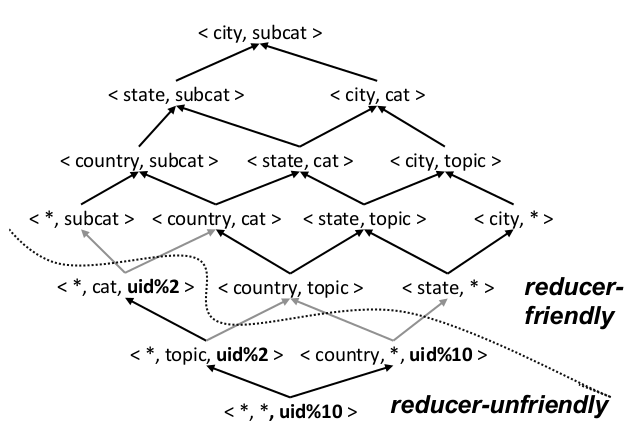
\includegraphics[width=4in]{picture/ch_datacube_mr/region_partition} 
\caption{根据uid被划分的lattice}\label{region_partition} 
\end{figure} 

上述的方法之所以会对一个 region 内的所有的 group 划分,是因为 region 的数量远比 group 少得多,若要记录所有的 group 是否需要划分,需要太大的开销。这样的方法能将大 group 划分,但 region 中只有 1 个 group 是 unfriendly 的,其他的group 仍要被迫划分,这样导致不必要的划分以及出现过多的被划分数据,加重了最后的合并操作。同时,论文中使用了求余的方式进行划分,这样的哈希方式非常简单,在很多情况下也是有效的,但是在一些极端的情况下,也可能导致划分的不均匀。就以上两点不足,这样的划分方式仍有可改进的空间。

\subsection{Batch Area}

对于中间数据过多的问题,MR-Cube中提出了 Batch Area 的概念。也就是利用 region 之间的父子关系,将多个 group 放在同一个 reducer 中计算,而不是像 Naive 的方法,一个 reduce 只计算一个 group。论文中给出了划分 batch 的一些规则,规则包括以下几点。
\begin{itemize}
\item reducer-unfriendly 的 region 和 reducer-friendly 的 region 不可划分在同一个batch内。
\item Reducer-unfriendly region 的划分,同一个 batch 内的 region 需要有相同的划分因子。
\item 同一个 batch 中的 region 需要有父子关系。
\item 两个 batch 的 region 数量差别不能超过2。
\end{itemize}

图\ref{batch_area}是其中一种合乎规则的划分方式。相同颜色的表示在同一个 batch 内。 

\begin{figure}[!htbp] 
\centering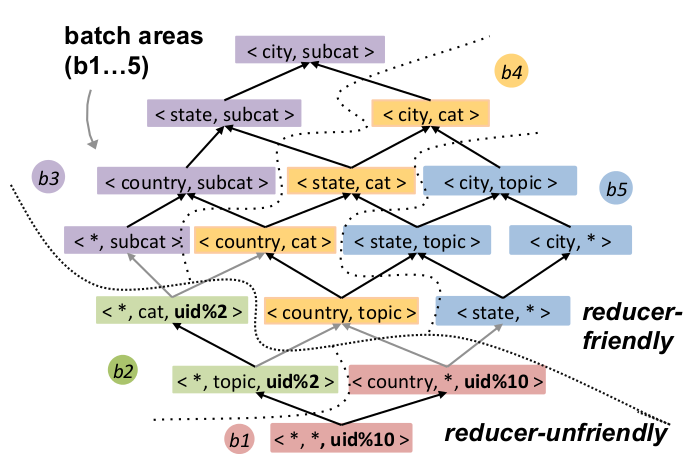
\includegraphics[width=4in]{picture/ch_datacube_mr/batch_area} 
\caption{Batch Area}\label{batch_area} 
\end{figure}

对于同一个 batch 内的 group 要如何计算有很多方法,论文使用的是BUC,(bottom up cubing algorithm)。但这种方法可能需要对数据扫描多次,而 MapReduce 的 reduce 中提供的迭代器仅能对数据扫描一次,若要对数据进行多次扫描,则需要载入内存中。并且 BUC 这种方法也未充分利用 MapReduce 框架的优势,例如排序功能。因此这里可以考虑替换其他的方法。同时,论文中只给出了batch 划分的规则,和提到可用贪心或者模拟退火的方式找出合乎规则的 batch,并没有给出具体的方法,而模拟退火这样的计算方法又稍微复杂。因此这里可以考虑在遵循规则的情况下,提出简单而有效的划分方法。


\section{贡献与不足}

MR-Cube \cite{nandi2011distributed} 这篇论文对使用 Naive 算法计算数据立方中存在的问题提出了一些非常有效的改善方法,论文的主要贡献包括:

\begin{enumerate}
\item 提出了对整体性度量划分的方式。
\item 提出了如何确定 group 是需要划分的,以及其划分的方法。
\item 提出了将多个 region 合并一起计算的 batch area 的概念。
\end{enumerate}

但是以上的方法也存在一些问题。

\begin{enumerate}
\item 论文中通过 region 内的一个大 group 将一个 region 内的所有 group 都贴上 reducer-unfriendly 的标签,导致 region 内所有的 group 都要划分。有些情况下可能一个 region 就只有一个大 group,而其他的 group 都很小,这样就导致了不必要的划分。
\item 求余(\%)是使用进行数据划分的方式,也就是一种 hash 方法,但是这种 hash 方法在一些极端情况下,可能会导致划分不均匀。
\item Batch area 内的计算,也就是多个 group 之间的计算,论文里使用的 BUC 的方法,虽然这种方法很合适有条件限定的情况(例如 HAVING),但是并没有很好地利用 MapReduce 本身的一些优势,例如排序。
\item 论文中只给出了 batch area 的规则,并没有提供简单且能满足规则的划分方法。
\end{enumerate}

因此接下来针对以上4点,使用 Tera-Sort 与 PipeSort 的方式对 MR-Cube 进行改进。





